\documentclass[a4paper]{article}

\usepackage{amsmath}
\usepackage{hyperref}
\usepackage{biblatex}
\usepackage{enumerate}
\usepackage{graphicx}
\usepackage{stmaryrd}
\usepackage[dvipsnames]{xcolor}
\usepackage{listings}
\usepackage{float}
\addbibresource{refs.bib}

\begin{document}

\author{
  Sebastian Miles \\
  \href{mailto:miless@chalmers.se}{miless@chalmers.se}
  \and
  Olle Lapidus \\
  \href{mailto:ollelap@chalmers.se}{ollelap@chalmers.se}
}
\title{DAT565/DIT407 Assignment 6}
\date{2024-10-11}

\maketitle
\section*{Problem 1}
We verify that the images are 28x28 pixels grayscales and plot a few of the images.
\begin{figure}[H]
	\begin{center}
		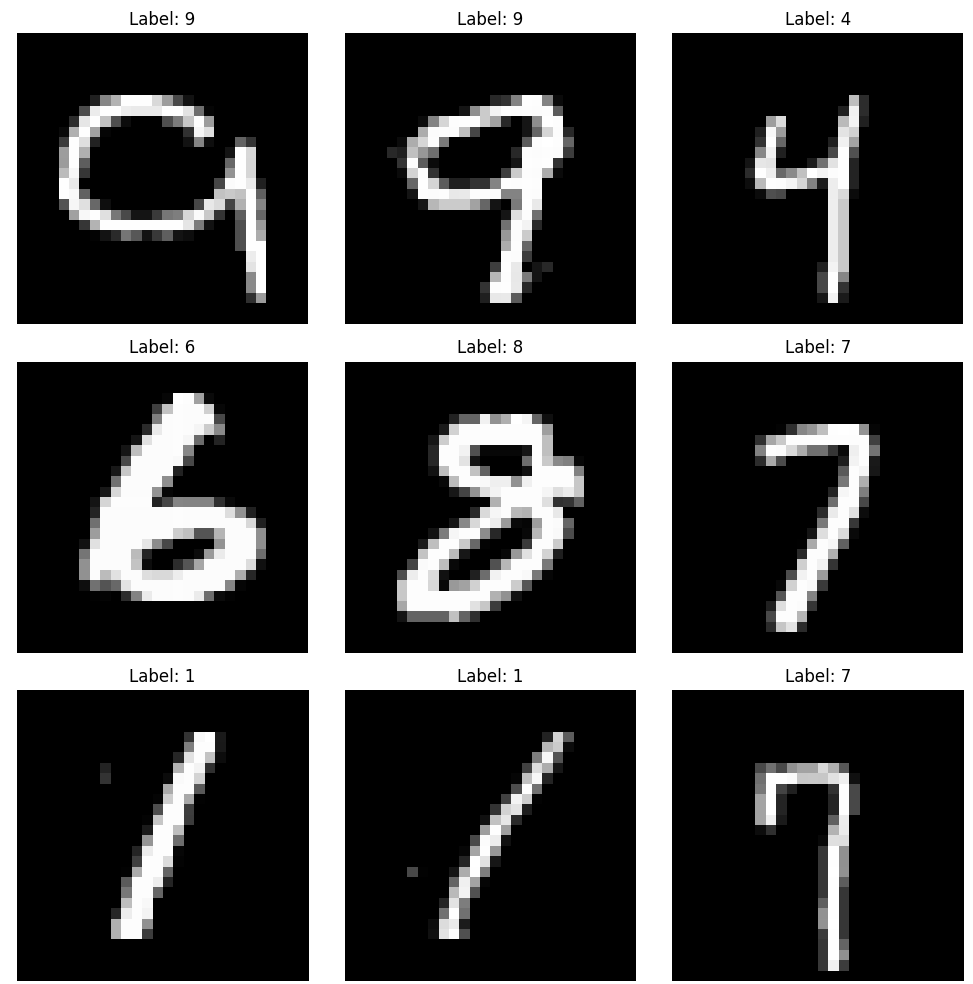
\includegraphics[scale=0.25]{datasets.png}
		\caption{Various images from the datasets}
		\label{hist}
	\end{center}
\end{figure}

\section*{Problem 2}
We train the data with a single hidden layer. We put the hidden layer size as 128 and the learning rate for the SGD as 0.01. The accuracy over 10 epochs is shown in figure \ref{tab}.
\begin{table}[h!]
	\centering
	
	\begin{tabular}{|c|c|}
		\hline
		Epoch & Accuracy \\
		\hline
		1 & 79.45\% \\
		\hline
		2 & 82.06\% \\
		\hline
		3 &  84.35\%\\
		\hline
		4 &  83.96\%\\
		\hline
		5 &  84.61\%\\
		\hline
		6 &  85.36\%\\
		\hline
		7 &  84.10\%\\
		\hline
		8 &  85.57\%\\
		\hline
		9 &  84.92\%\\
		\hline
		10 &  86.75\%\\
		\hline
	\end{tabular}
	\caption{Accuracy of the test data over 10 epochs. }
	\label{tab}
\end{table}

\section*{Problem 3}

\subsection*{MultinomialNB}

\begin{table}[h!]
    \centering
    \begin{tabular}{|c|c|c|c|}
        \hline
        & Predicted Ham & Predicted Spam & Sum \\
        \hline
        Actual Ham & 1281 & 1 & 1282 \\
        \hline
        Actual Spam & 73 & 171 & 244 \\
        \hline
        Sum & 1354 & 172 & 1526 \\
        \hline
    \end{tabular}
    \caption{Confusion Matrix for MultinomialNB}
    \label{mNB}
\end{table}


See table \ref{mNB}\\
\textbf{Precision} (ham): 0.95 \\
\textbf{Precision} (spam): 0.99 \\
\textbf{Recall} (ham): 1.00 \\
\textbf{Recall} (spam): 0.70

\subsection*{BernoulliNB}
\begin{table}[h!]
	\centering
	\begin{tabular}{|c|c|c|c|}
		\hline
		& Predicted Ham & Predicted Spam & Sum \\
		\hline
		Actual Ham & 1280 & 2 & 1282 \\
		\hline
		Actual Spam & 180 & 64 & 244 \\
		\hline
		Sum & 1460 & 68 & 1528 \\
		\hline
	\end{tabular}
	\caption{Confusion Matrix for BernoulliNB}
	\label{bNB}
\end{table}
\noindent
See table \ref{bNB}\\
\textbf{Precision} (ham): 0.88 \\
\textbf{Precision} (spam): 0.97 \\
\textbf{Recall} (ham): 1.00 \\
\textbf{Recall} (spam): 0.26\\\\
The classifier demonstrates high accuracy, with a precision of 0.99 for spam detection, although the recall for spam is somewhat lower, indicating occasional missed spam emails.

\section*{Problem 4}

\printbibliography
\appendix

\section*{Code}
\label{app:excode}

\lstset{
	language=Python,
	basicstyle=\ttfamily,
	commentstyle=\color{OliveGreen},
	keywordstyle=\bfseries\color{Magenta},
	stringstyle=\color{YellowOrange},
	numbers=left,
	frame=tblr,
	breaklines=true,
	postbreak=\mbox{\textcolor{red}{$\hookrightarrow$}\space},
}
\begin{lstlisting}

\end{lstlisting}

\end{document}
